\Cref{fig:additional_figures} shows some additional analyses of the parameter landscape.
\begin{figure}[ht!]
  \centering
  \begin{subfigure}{0.3\textwidth}
    \centering
    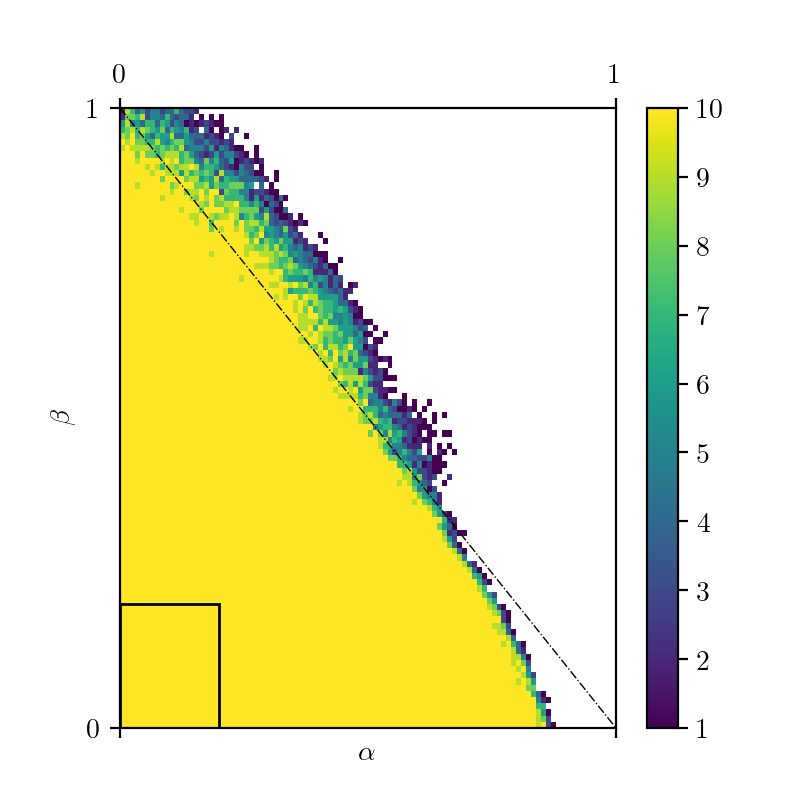
\includegraphics[width=\textwidth]{figure/physical_runs}
    \caption{Physical runs}
    \label{fig:physical_runs}
  \end{subfigure}%
  \begin{subfigure}{0.3\textwidth}
    \centering
    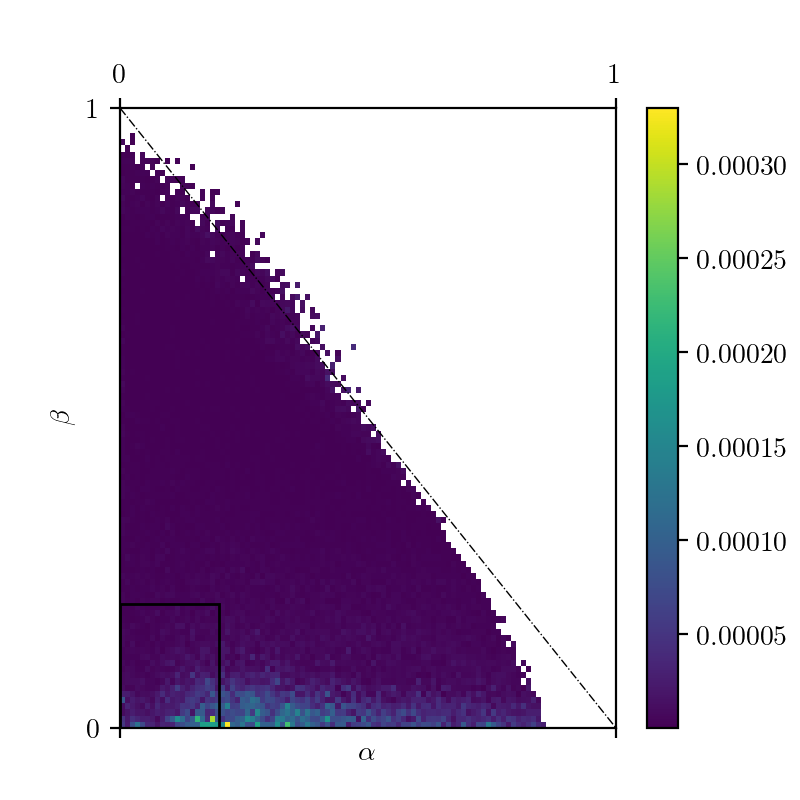
\includegraphics[width=\textwidth]{figure/chimera_var}
    \caption{Chimera variance}
    \label{fig:chimera_var}
  \end{subfigure}%
  \begin{subfigure}{0.3\textwidth}
    \centering
    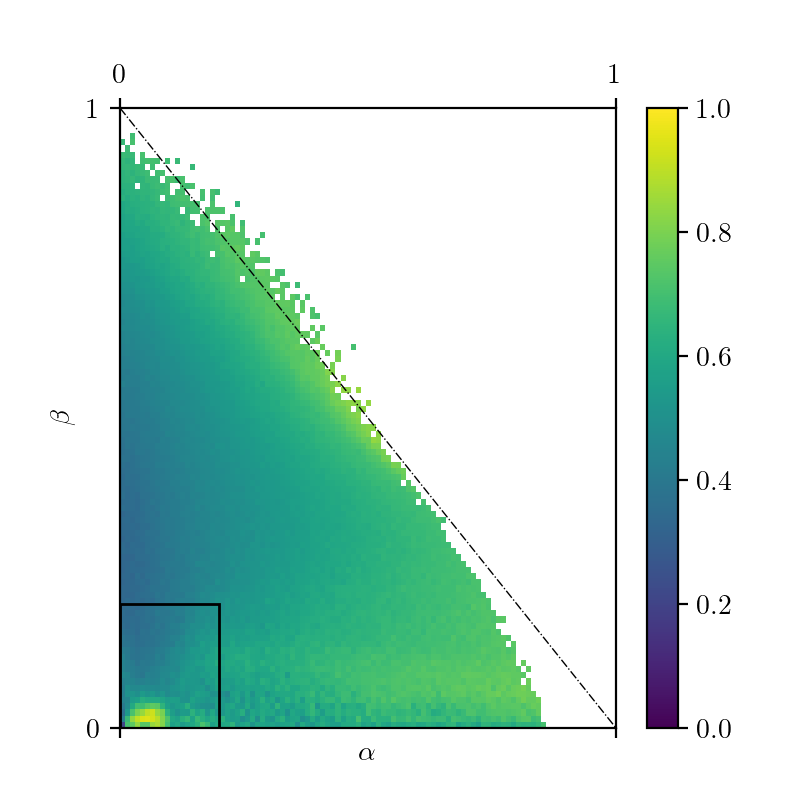
\includegraphics[width=\textwidth]{figure/meta}
    \caption{Metastability}
    \label{fig:meta}
  \end{subfigure}
  \begin{subfigure}{0.3\textwidth}
    \centering
    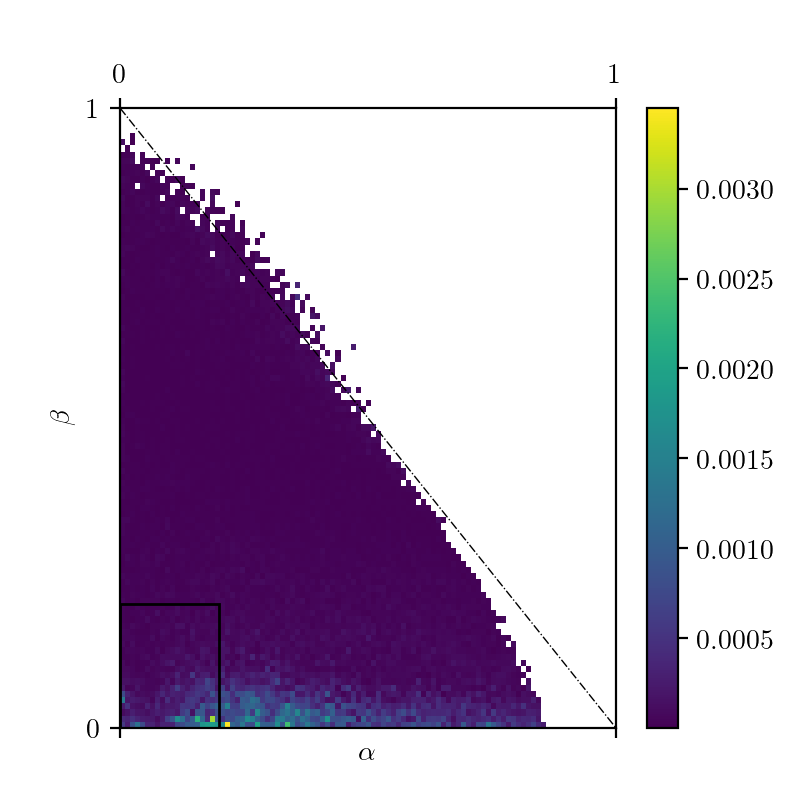
\includegraphics[width=\textwidth]{figure/meta_var}
    \caption{Metastability variance}
    \label{fig:meta_var}
  \end{subfigure}%
  \begin{subfigure}{0.3\textwidth}
    \centering
    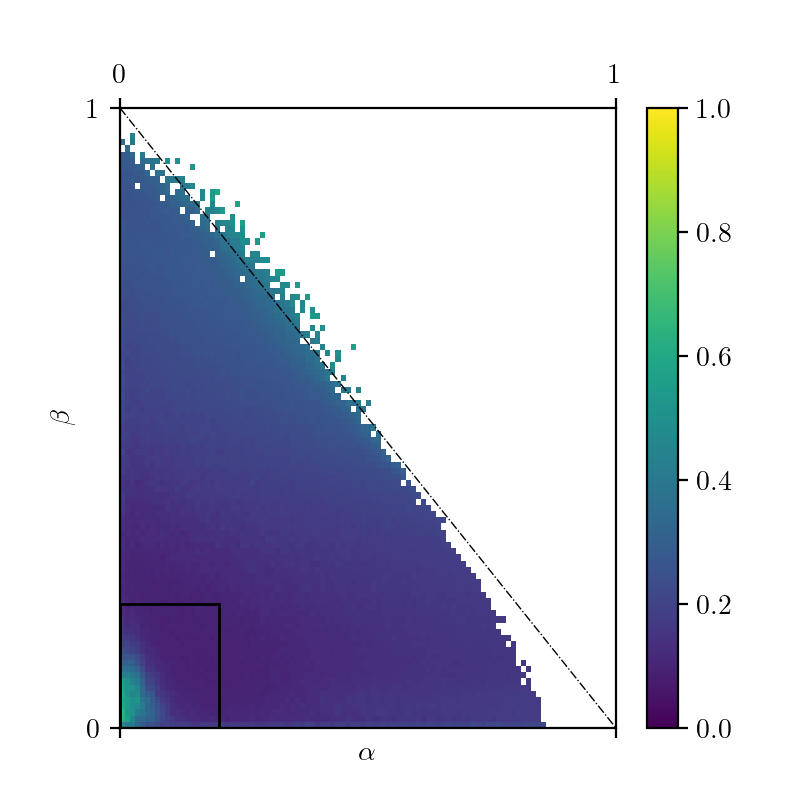
\includegraphics[width=\textwidth]{figure/r}
    \caption{$r$}
    \label{fig:r}
  \end{subfigure}%
  \begin{subfigure}{0.3\textwidth}
    \centering
    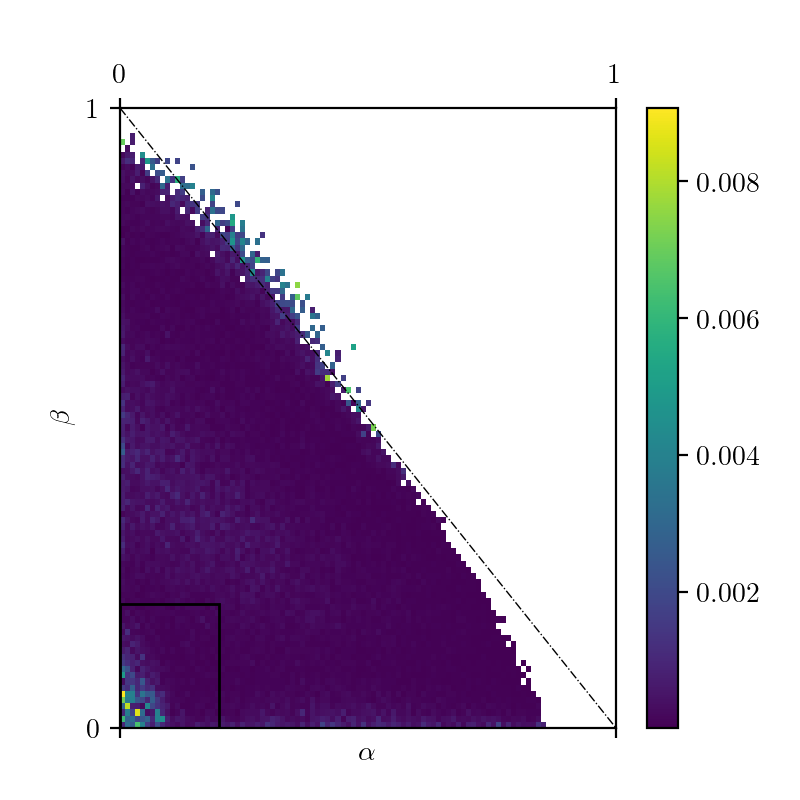
\includegraphics[width=\textwidth]{figure/r_var}
    \caption{$r$ variance}
    \label{fig:r_var}
  \end{subfigure}%
  \caption[Additional figures]{Additional analyses of the parameter landscape.
    \Cref{fig:physical_runs} shows the number of runs (out of 10) which gave physical results.
    All parameter sets which are not yellow in \cref{fig:physical_runs} were excluded from the other analyses.
    \Cref{fig:chimera_var} shows the variance of the chimera-like index.
    \Cref{fig:meta} shows the metastability index.
    \Cref{fig:meta_var} shows the variance of the metastability index.
    \Cref{fig:r} shows the mean order parameter over time, averaged across runs.
    \Cref{fig:r_var} shows the variance between runs of the mean order parameter.
  }
  \label{fig:additional_figures}
\end{figure}

%%% Local Variables:
%%% mode: latex
%%% TeX-master: "../ms"
%%% End:
